\chapter{User interface}

A \emph{user interface} (UI) is the front-facing part of Pepr3D that the users interact with.
It is responsible for managing windows, showing buttons, rendering the 3D model, handling mouse clicks, hotkeys, showing error dialogs, and much more.
In case of Pepr3D, it should be an easy-to-use, intuitive, and fast abstraction of the complex 3D geometric algorithms at the backend, see Figure~\ref{fig:diagram_ui}.

\medskip

We divide the Pepr3D UI into the following main parts:
%
\begin{itemize}
\setlength\itemsep{0em}
\item the \textbf{main application} corresponds to the whole main window, which consists of the following:
\item a \textbf{toolbar} with toggleable buttons representing tools, undo/redo, etc.,
\item a \textbf{side pane} with buttons, checkboxes, sliders, etc., representing configuration of the currently selected tool,
\item and a \textbf{model view} with the 3D model which the user can rotate, zoom, paint on it, etc.
\end{itemize}

\begin{figure}[h]
	\centering
	\centerline{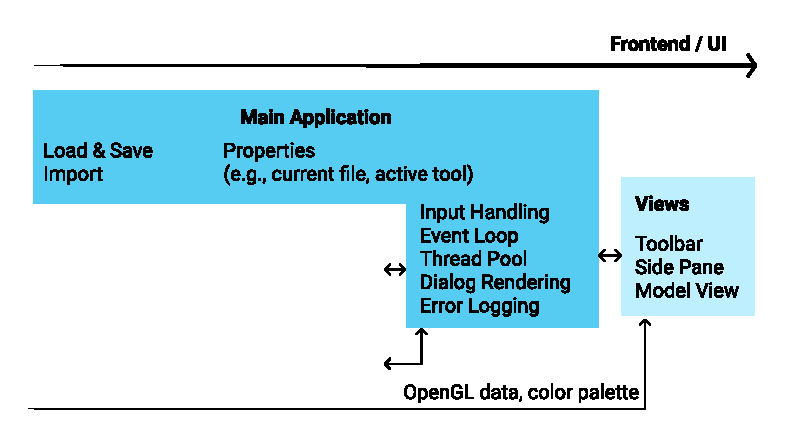
\includegraphics[scale=1.0]{images/diagram_ui.eps}}
	\caption{An overview of the Pepr3D UI architecture, based on Figure~\ref{fig:architecture}.}
	\label{fig:diagram_ui}
\end{figure}
\vspace{-1.5em}

\section{Key concepts}

In the specification of Pepr3D, we explained several main ideas that the user interface of Pepr3D is built around.
We will not repeat every single idea from the specification here as that would be redundant, but we explain the key concepts that we kept in mind while developing the user interface.

To prevent reinventing the wheel, our concepts are based on investigating how other developers implement user interfaces.
Our UI mainly consists of \emph{real-time 3D rendering}, i.e., displaying the 3D model that users can interact with, and \emph{widgets}, i.e., the windows, buttons, check boxes, text labels, etc.

\subsection{Real-time 3D rendering}

In Pepr3D, a regular user interface with a few buttons and texts is not enough.
We primarily need real-time 3D rendering and manipulation of the 3D model that the user is editing.
Hence the whole user interface needs to take this into account and is primarily based on real-time rendering.

As explained in our specification, when we were looking for a 3D rendering library, we mainly focused on finding an easy-to-use abstraction, e.g., for rendering 3D primitives, using custom shaders with uniforms, uploading textures to the GPU, keeping constant framerate, etc.
We decided to use \emph{Cinder}, which is also cross-platform and supports asynchronous events.

\subsection{Widgets}

As Pepr3D is based on real-time rendering, we decided to use \emph{immediate UI}, i.e., a procedural UI redrawn every frame that is mostly stateless.
This means that we do not have to program any explicit synchronization between the UI and the backend.
Whenever we rerender the UI, it will be rendered with the newest data.
Retained state is only where necessary, e.g., for complex calculations not needed in every frame.
Our immediate UI is a part of the 3D renderer based on Cinder and OpenGL, where the widgets are rendered on top of the scene.

We also kept in mind that \emph{presentation should be separated from the logic}, i.e., the rest of the application should know nothing about the UI at all.
Hence our UI depends on the backend, but the backend does not depend on the UI at all.
In theory, we are able to easily replace the UI with another, should it be necessary.

For these reasons and others explained in our specification, we based our widgets on a library called \emph{Dear ImGui}.
It provided us with basic handling of mouse clicks, keyboard inputs, etc., and also with 2D drawing such as texts, icons, buttons, etc.
But the design of Pepr3D is completely ours and is based on heavily customized widgets based on ImGui primitives.

\section{Application}

The whole application and its main window are executed via the Cinder library.
The main file \texttt{main.cpp} contains a Cinder macro which corresponds to cross-platform \texttt{main} functions.
Cinder is responsible for creating an instance of our \texttt{MainApplication} class on which it calls the \texttt{setup} method.

After the main window is set up, Cinder keeps calling the \texttt{update} and \texttt{draw} methods every frame in this order.
Cinder also handles all necessary events from an operating system and calls the appropriate methods of the \texttt{MainApplication}.

\subsection{Main application}

The \texttt{MainApplication} class is a router which interacts with other components, mainly the three major UI components: a \textbf{toolbar}, a \textbf{side pane}, and a \textbf{model view}.
It instantiates them, listens for events from the operating system, and passes them to the components so that they can handle them themselves.

This also includes delegating hotkeys, open, save, import, and export commands to their dedicated classes, handling minimized application, etc.
We can say that every user interaction gets first through the \texttt{MainApplication} which then delegates it to other components.

Because of the Cinder API, setup is not done directly in the constructor, which only instantiates other components, but in the \texttt{setup} method which Cinder calls once it is ready.
It creates and configures debug and error loggers, sets the main window properties such as its resolution and icon, initializes ImGui, hotkeys, the default geometry (cube), and constructs all tools.

The \texttt{draw} method draws the major UI components and also renders existing modal dialogs and a progress indicator when necessary.
The \texttt{update} method checks invariants such as that the selected tool is not disabled, application is not rendered if minimized, and unsaved changes in a project are marked with an asterisk * in the title.

\subsection{Multithreading and background tasks}

Some operations such as importing or exporting a large model may take a long time.
If everything was done in the main thread, rendering of the UI would be paused and the window would become unresponsive.
In UI applications, we want to avoid this by running slow operations in the background.

For this purpose, we use a very simple thread-pool library consisting of just a single \texttt{ThreadPool} class.
A single instance of this thread pool is stored as a static member of the \texttt{MainApplication}.

Delegating a task into the thread pool is done by calling \texttt{enqueue} on the thread pool.
This method returns a C++ \texttt{future} which we can wait for.
However, the UI in the main thread should \emph{not} wait for the tasks to finish in a blocking way, as that would defeat the purpose.

Instead, we can call \texttt{dispatchAsync} on the \texttt{MainApplication}, which dispatches another callback via Cinder.
This callback will be executed before a new frame starts rendering.
This enables the background tasks to notify the UI that they have finished.

In summary, the pipeline works like this: the UI enqueues a slow function $F$ (typically a lambda function) to the thread pool and continues rendering.
Right before $F$ finishes, the $F$ itself calls \texttt{dispatchAsync} with another function $A$, which will be run on the UI thread at a new frame.
$A$ is used to update the UI to the new state, e.g., after loading a new model.

\subsection{Resources of a minimized or obscured window}

Because Pepr3D runs at a vertically synchronized framerate (typically 60 frames per second), it uses CPU and GPU resources even when minimized or obscured.
We had to implement a way to pause rendering while the window is not visible.
Cinder provided a way to tell if the window was minimized, but it did not solve situations where a window was obscured but not technically minimized.

This proved to be a difficult problem that we managed to partially solve for Microsoft Windows by using the Windows API.
In regular intervals, we check whether the top left corner, center, and bottom right corner are obscured by another window of another application.
When they are, we pause the rendering.
This significantly lowers the CPU and GPU usage when Pepr3D is not used.

\subsection{Dialogs and fatal error handling}

In Pepr3D, there are 3 types of dialogs: general modal dialogs, a special export dialog, and a progress indicator.
All these dialogs are drawn from the \texttt{MainApplication} on top of everything else and all mouse and keyboard input for the rest of the components is paused.

\paragraph{General modal dialogs and fatal errors}
General modal dialogs are represented by the \texttt{Dialog} class and they can be of various importance, e.g., information dialogs, fatal error dialogs, etc.
The dialogs are stored in a priority queue with the most important dialog on top.
They can be pushed to the queue by calling \texttt{pushDialog} on the \texttt{MainApplication} instance.

When we detect an invalid state of the application, e.g., by catching a fatal exception, a \emph{fatal error dialog} is pushed to the queue.
When a fatal error dialog is on the top of the queue, rendering of all components is stopped and only the dialog is shown, because it cannot be guaranteed that other components are in a valid state.
Pressing a button on the fatal error dialog terminates the application.

Sometimes an error is so fatal that even the fatal error dialog cannot be rendered and Pepr3D is terminated immediately.
Nevertheless, all warnings, errors, and fatal errors are logged in \texttt{pepr3d.log} files which are backed up in case of a fatal error.
When Pepr3D is executed again, an information dialog is shown explaining the user where they can find a related log file with error details.

\paragraph{Export dialog}
An export dialog is a complex dialog shown when a user attempts to export a model.
Because it contains a lot of buttons and options, it is handled separately directly by the \texttt{MainApplication}.

\paragraph{Progress indicator}
A progress indicator is an animated dialog which shows the elapsed and remaining progress required to process the current command.
It is used mostly when opening, saving, importing, and exporting geometry files, because this is a slow process.
Its logic is handled in the \texttt{ProgressIndicator} class which has a pointer to the \texttt{Geometry} which is being loaded.
The current status is checked directly from the geometry data every frame.

\subsection{Tooltips}

As the user interface has to be as clean as possible to allow fast and easy navigation even for beginners, long and detailed explanations of buttons and input boxes are ``hidden'' in tooltips.
Tooltips are black rectangles with information that display when user hovers over an interactive widget, e.g., a button.

Tooltips in Pepr3D can show a name of an action, its hotkey (if available), long description of an action (if provided), and an explanation why an action is disabled (if it is disabled).
Tooltips are created by calling \texttt{drawTooltipOnHover} on the \texttt{MainApplication} instance.
They are only drawn when the item is actually hovered.

\subsection{Hotkeys}

Hotkeys (keyboard shortcuts) enable users to perform common actions by pressing a single key or a combination of keys.
Using hotkeys, changing active tools and colors is much faster and so is the whole editing process.
There is no need to move a mouse cursor over the whole window just to change a color and then move back over the edited geometry.

Hotkeys are managed by the \texttt{Hotkeys} class which contains a mapping between \texttt{Hotkey} and \texttt{HotkeyAction}.
There are two maps, one for each direction, i.e., a hotkey to action, and an action to a hotkey.
The former one is used for faster event handling, the later one for faster displaying of tooltips that show what keys to press.

A \texttt{Hotkeys} instance is managed by the \texttt{MainApplication} which loads user specified hotkeys from a file in \texttt{assets/hotkeys.json}.
If this file does not exist, default hotkeys are loaded.
When a key is pressed, \texttt{MainApplication} calls \texttt{findAction} on the \texttt{Hotkeys} instance and then performs the corresponding action.
Similarly, \texttt{Toolbar} and \texttt{SidePane} call \texttt{findHotkey} on the \texttt{Hotkeys} instance to find which key should be shown in a tooltip.
The \texttt{getString} method on a \texttt{Hotkey}, unfortunately, only supports letters and numbers and a \texttt{Ctrl+} modifier.
There is no mapping between key codes and UTF-8 symbols.

Hotkeys are customizable, but only by editing the file \texttt{assets/hotkeys.json}.
The file has a simple JSON structure as can be seen in the example:

\begin{lstlisting}
{
    "hotkeys": {
        "keysToActions": [
            {
                "key": {
                    "ctrl": false,
                    "keycode": 100
                },
                "value": "SelectDisplayOptions"
            },
            {
                "key": {
                    "ctrl": false,
                    "keycode": 101
                },
                "value": "SelectTextEditor"
            },
            ...
        ]
    }
}
\end{lstlisting}
where the key codes are based on Cinder and can be found in the user documentation.

\section{Toolbar and side pane}

The toolbar and side pane are two major UI components that users interact with.
They are both rendered on top of the geometry, covering the top and right part of the window.

\subsection{Toolbar}

The toolbar is represented by the \texttt{Toolbar} class.
It is rendered on the top of the window and meets with a side pane at the right side.
It consists of 3 main parts: the file drop down on the left, the undo and redo buttons, and the tool buttons that select active tools.

All the buttons in the toolbar are rendered via the templated \texttt{drawButton} method.
It is a heavily modified ImGui button, because our toolbar buttons also support multiple states (inactive, hovered, held, active, disabled) and a dropdown option which we use for the file drop down.

The tool buttons are not hard-coded, but rendered by dynamically iterating over all \texttt{Tool} instances that are part of the \texttt{MainApplication}.
For example, when we compile in the debug mode, there is an additional debug tool, which is not present in the release version.

\subsection{Side pane}

The side pane is represented by the \texttt{SidePane} class.
It is rendered on the right side of the window and fills up the whole height of the screen.
It consists of 2 main parts: the header which shows the currently active tool, and the ``inside'' where properties of the active tool are shown.

There is an important concept: \emph{the tools themselves draw the inside of the side pane}.
The side pane only calls the \texttt{drawToSidePane} method on the currently active \texttt{Tool} and the \emph{tool itself} decides what is drawn by calling \texttt{SidePane} helper methods such as \texttt{drawText}.

So it is the side pane which knows how to draw texts, buttons, color palette, separators, and other UI widgets in the side pane, but what exactly gets drawn is decided by the tools.
This is a design decision that makes the \texttt{SidePane} independent on the specific tools and enables them to provide various properties that the users can edit in real-time.

\paragraph{Standard widgets}
Side pane can contain standard widgets.
These are for example texts drawn by \texttt{drawText}, buttons and colored buttons by \texttt{drawButton} and \texttt{drawColoredButton}, separators by \texttt{drawSeparator}, checkboxes by \texttt{drawCheckbox}, and more.
The tools can, however, also use ImGui directly, because all ImGui calls from inside their \texttt{drawToSidePane} method get automatically associated with the side pane.

\paragraph{Color palette}
The most complex widget available in the side pane is the color palette.
This is an advanced and completely custom widget built using basic ImGui components.

It has two modes: the ``read-only'' color palette only shows color boxes that can be clicked and selected, the ``editable'' mode allows the user to completely customize the color palette of Pepr3D.
The former is shown in most tools such as triangle painter or brush, the later is used in Pepr3D settings.

The color palette is synchronized with the \texttt{ColorManager} directly.
The editable mode consists of 4 parts: the header, the ``add'' button and ``delete'' box, the color boxes (also present in the read-only mode), and a ``reset'' button.

The drag-and-dropping feature is using the ImGui experimental API built for these purposes.
The color boxes hold a payload with their IDs and when they are dropped on a different color box, the colors get swapped or reordered.
The difference between swapping and reordering is that the former also swaps the colors in the geometry, while the later only reorders them in the palette.
When a color box is dropped on the ``delete'' box, the color is removed entirely from the geometry and replaced by the first color in the palette.

\section{Model view}

The model view is the 3D part of the UI, represented by the \texttt{ModelView} class.
It is responsible for rendering the geometry and allowing users to interact with the active tool by clicking and dragging over the geometry.
It also handles the camera, i.e., moving around the model, and shows an optional grid representing the printing bed and a wireframe consisting of the triangles of the model.

\subsection{Model matrix scaling, translations, and rotations}
Before even drawing the model, we must first handle its dimensions, position, and rotation.
This is because different models, especially models imported from different 3D editors, have various scales and origin points.

We made an \texttt{updateModelMatrix} method responsible for scaling, translating, and rotating the geometry with regards to the following rules.
The model's largest dimension in the XYZ axes must be $1.0$, so that the whole model is visible on the screen without the need to zoom in or out.
This is done by computing the axis-aligned bounding box (AABB) of the model and using its dimensions.

The model is also translated so that it is centered over the $(0,0,0)^T$ point
But the lowest edge of the model must touch the grid at height $y=0$, so we need to translate in the $y$ axis again, moving the model up a little bit.

Finally, we rotate the model so that the $z$ axis points up, because this is the standard in 3D printing pipelines and corresponds to what the slicer uses.
This is different than in OpenGL where the $y$ axis is usually considered to be the up axis.
This rotation also means that what users can see in Pepr3D corresponds to what they can see in Blender or Slicer for Prusa printers.

\subsection{Drawing geometry}

Drawing the current \texttt{Geometry} instance is the main responsibility of the model view.
The \texttt{draw} method consists of several steps that we now describe.

First it sets up the OpenGL viewport to only render to the model view part of the window, i.e., to ignore the toolbar and side pane parts.
Then we push the camera matrices to OpenGL, which sets up the position and direction from which we look at the model.

Then the \texttt{updateModelMatrix} method is called and the model matrix is updated.
The scaling, translations, and rotations only happen during the rendering, so the original geometry is not affected at all.

Then we call the \texttt{drawGeometry} method, which uploads all necessary data to the GPU via OpenGL.
We push the model matrix, update vertex buffer objects, update shader uniforms, and finally draw the batch using OpenGL vertex and fragment shaders.
Note that the vertex and index buffers may be very large and may update every frame.
For these reasons, we do two optimizations.

First, the buffers are only uploaded when a change is detected.
This is handled in the \texttt{Geometry::OpenGlData} class which also stores the data on the CPU side.
The second optimization is that we do not upload the colors of the model directly to the vertices, instead every vertex has an index to the palette.
The color palette itself is uploaded to the GPU as a uniform array and then it is used in the fragment shader.

After drawing the geometry, we also draw the grid that simulates the printing bed of the printer.
One cell of the grid measures $0.1\times{}0.1$, the whole grid is $1.8\times{}1.8$, so that it is always slightly bigger than the model itself.

\subsection{Shaders}

In order to display the geometry, we need to provide the GPU with two OpenGL shaders written in GLSL.
The vertex shader is called on every vertex of a triangle of the model.
The fragment shader is then called on every single fragment (pixel) of the displayed model.
This is a standard OpenGL pipeline.

In the vertex shader located in \texttt{assets/shaders/ModelView.vert}, we primarily just forward vertex attributes to the fragment shader.
Additionally, we also generate barycentric coordinates of the vertex.
This uses the fact that OpenGL interpolates attributes over the triangles, so if we set the barycentric coordinates in the vertices, they are automatically correctly interpolated for the fragment shader.

In the fragment shader located in \texttt{assets/shaders/ModelView.frag}, we need to calculate the final color of every fragment.
There are several steps that contribute to the color.
Primarily, we use Lambert shading to display the model, where we assume the light source always points from the camera.
The main color of the model is found in the color palette with regards to the ID attribute of the vertex.

In case the brush tool is active, we also calculate whether the current fragment is inside the highlighted region of the brush.
And finally if the wireframe rendering is enabled, we use the interpolated barycentric coordinates from the vertex shader to find out whether we are on an edge of a triangle, and if so, we highlight it in a contrast color.

\subsection{Camera}

While painting the model, users of Pepr3D need to rotate and zoom the model in order to paint details from all sides of the geometry.
Typically, in all major 3D editors, a so called arc-ball camera is used.
The camera moves around a pivot point (the model in our case) by dragging the mouse on the screen.
Zooming is usually performed with the mouse wheel.
Other actions may also be performed and are explained in the user documentation.

We originally used a camera implementation from Cinder called \texttt{CameraUi}.
Unfortunately, during our testing, we found out that their implementation of zooming is not perfect for all our purposes.
We modified the original \texttt{CameraUi} so that it supports two types of zooming.

Now, \emph{zoom} in our case means changing the field of view of the camera.
\emph{Dolly}, on the other hand, means moving the camera position towards or further away from the pivot point (the model).
We also fixed a bug in which dollying too close would move the pivot point and cause unexpected behavior.